\section{Implementierung des Backends}

In diesem Kapitel wird die technische Umsetzung der Applikation beschrieben. Neben der Projektstruktur werden zentrale Komponenten der Implementierung, darunter das Backend, die API-Schnittstellen sowie Sicherheitsmaßnahmen, vorgestellt. Zudem werden Herausforderungen und Lösungsansätze erläutert.

\subsection{Projektstruktur und Überblick}

\subsubsection{Versionierungssoftware}

Für das Projekt wird das Versionierungssystem \texttt{git} verwendet. Dieses wird auf der Plattform namens Github (siehe \cite{website-github}) zur Verfügung gestellt und bietet damit eine optimale Entwicklungsumgebung. Für das Backend wurde ein separates \texttt{Repository} erstellt, welches unter folgender URL aufgerufen werden kann: \cite{website-git-backend-repo}. Alle Dateien, welche im Rahmen dieser Arbeit genauer untersucht und beschrieben werden, sind in diesem Repository auffindbar.

\subsubsection{Projektstruktur}

Das eigentliche Projekt unterteilt sich in die folgenden Hauptpakete:

\begin{itemize}
	\item \textbf{Controller}: Hier werden die Kontrollelemente der Applikation, damit unter anderem die REST-Schnittstellen programmiert.
	\item \textbf{Model}: In diesem Paket sind alle Datenstrukturen enthalten, welche für das Backend benötigt werden.
	\item \textbf{Repositories}: Hier befinden sich die jeweiligen Repositories zu den Model-Files, damit auf diese CRUD-Operationen (\gls{crud}) angewendet werden können (dies ist eine Funktionalität, welche von der \gls{jpa} zur Verfügung gestellt wird).
	\item \textbf{Config}: In diesem Ordner befinden sich applikationsübergreifende Konfigurationen, wie zum Beispiel die Security-Configuration für unsere REST API.
	\item \textbf{Services}: Hierbei handelt es sich um ein Paket, in dem Service-Elemente für die Authentifizierung zu finden sind.
	\item \textbf{Utilities}: Hier können nach Bedarf Dateien bzw. Programme eingefügt werden, die nicht mit den anderen Paketen kategorisierbar sind, jedoch trotzdem einen fixen Platz im Ablauf haben.
	\item \textbf{Exceptions}: Hier wird die eigene Implementierung der globalen Exception-Handling Struktur gespeichert.
\end{itemize}

\subsubsection{Einrichtung des Projekts}

Um das Projekt einzurichten, wurde der Spring Initializr (siehe \cite{website-spring-initializr}) verwendet. 

Die grafische Oberfläche dieses Werkzeugs sieht folgendermaßen aus:

\begin{figure}
	\centering
	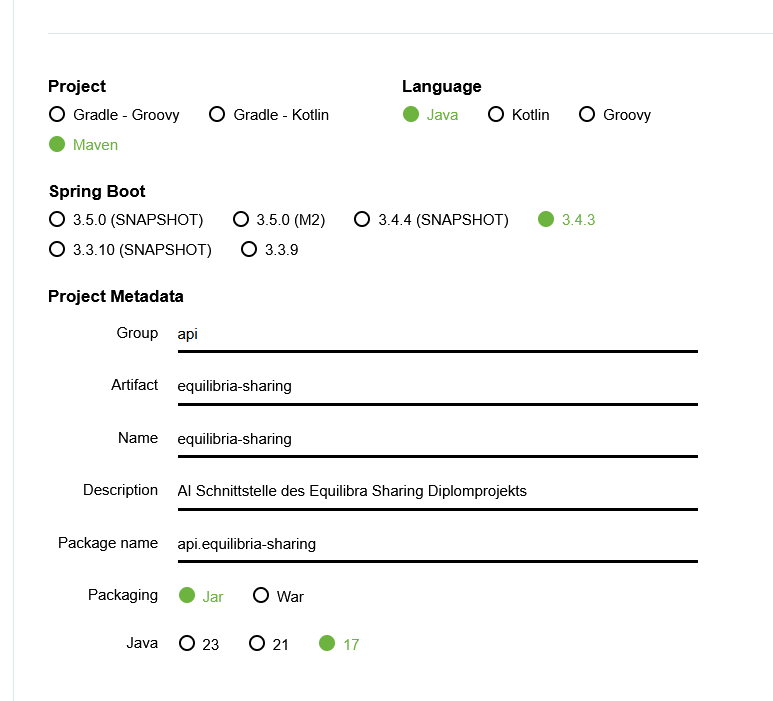
\includegraphics[width=1\textwidth]{images/impl-spring-init-1.png}
	\caption{Die grafische Darstellung des Spring Initializr. Hier werden allgemeine Projektdaten angegeben. \textit{\cite{website-spring-initializr}}}
    \label{backend-spring-init-1}
\end{figure}

In der Abbildung \ref{backend-spring-init-1} ist ein Teil der grafischen Oberfläche des Tools zu sehen. Hierbei können projektspezifische Daten, wie zum Beispiel der Name, die gewünschte Spring Boot Version, uvm. eingegeben werden.

\begin{figure}
	\centering
	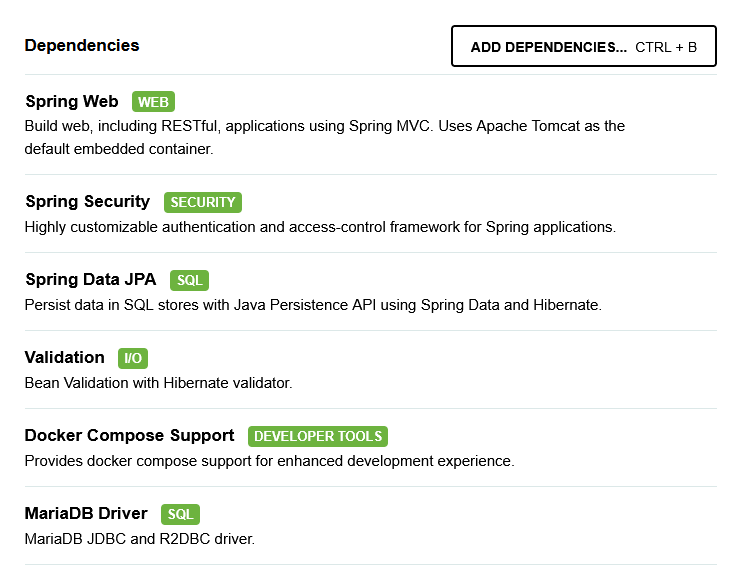
\includegraphics[width=1\textwidth]{images/impl-spring-init-2.png}
	\caption{Die grafische Darstellung des Spring Initializrs. In diesem Teil werden die gewünschten Pakete, welche im Projekt anfangs verwendet werden möchten, angegeben. \textit{\cite{website-spring-initializr}}}
    \label{backend-spring-init-2}
\end{figure}

Dieser Abbildung \ref{backend-spring-init-2} sind die jeweiligen Pakete, welche im Projekt anfangs verwendet wurden, zu entnehmen. Dabei können beliebige Pakete ausgewählt werden, welche bei der Generierung des Projekts automatisch eingebunden werden.

Nun wird ein ZIP-Archiv heruntergeladen, welches alle gewünschten Konfigurationen enthält. Dies bildet die Grundlage für das Equilibria Sharing Backend.

\subsection{API-Controller: Die Buchungsverwaltung}
\label{sec:apiDokumentation}
Die REST-Schnittstelle, welche die Verwaltung von Buchungen in der Anwendung bereitstellt, wird von dem sogenannten \texttt{BookingController} verwaltet. Hier befinden sich alle Endpunkte zum Erstellen, Abrufen, Aktualisieren und Löschen von Buchungen. Zudem sind Sicherheitsmechanismen zur Zugriffskontrolle implementiert. 

\subsubsection{Schnittstelle zur Datenbank}

Der Controller greift auf sogenannte \texttt{Repositories} zurück. Dies sind vorab definierte Interfaces, welche eine einfache Schnittstelle des Spring Boot Backends zur MariaDB-Datenbank ermöglichen. Damit lassen sich mittels Java-Quellcode Aktionen in der Datenbank ausführen.

Bei dieser API-Schnittstelle werden die folgenden Repositories verwendet:
\begin{itemize}
	\item \texttt{BookingRepository}: Verwaltung der Buchungseinträge
	\item \texttt{PersonRepository}: Speicherung der Reisenden
	\item \texttt{AccommodationRepository}: Verwaltung von Unterkünften
	\item \texttt{AddressRepository}: Speicherung von Adressen
\end{itemize}

Diese Repositories werden über den Konstruktor mithilfe der \gls{dependencyinjection} initialisiert (siehe \cite{website-spring-dependency-injection}):
\begin{lstlisting}[caption={Code-Ausschnit, welcher die Initalisierung aller notwendgen Klassen darstellt}, label={code-bookings-init}, language=Java]
	public BookingController(BookingRepository bookingRepository, 
	PersonRepository personRepository, 
	AccommodationRepository accommodationRepository,
	AddressRepository addressRepository) {
		this.bookingRepository = bookingRepository;
		[...]
	}
\end{lstlisting}

Damit werden direkt alle Schnittstellen zur Datenbank im Parameter des Konstruktors automatisch von Spring Boot mitgegeben und auch in die Klasse importiert.

Konkret müssen die Repositories jedoch noch folgendermaßen in der Klasse als Attribute hinterlegt sein:

\begin{lstlisting}[caption={Deklarierung der Repositories als finale (= nicht modifizierbare) Attribute.}, label={code-bookings-repositories}, language=Java]
	private final BookingRepository bookingRepository;
	private final PersonRepository personRepository;
	private final AccommodationRepository accommodationRepository;
	private final AddressRepository addressRepository;
\end{lstlisting}

Damit wird sichergestellt, dass die notwendigen Prozesse sorgfältig in der Datenbank abgearbeitet werden können.

\subsubsection{Erstellen einer Buchung}

Der Endpunkt \texttt{POST /api/v1/bookings} nimmt Buchungsanfragen entgegen. Die Methode \texttt{createBooking} validiert die Eingaben, speichert Hauptreisende, Adressen und Dokumente in der Datenbank und erstellt eine neue Buchung. Hierfür wird keine Authentifizierung benötigt, da die Aktion vom Benutzer ausgelöst wird. 

Bei dieser Anfrage ist die Angabe aller Buchungsdaten notwendig und im Normalfall auch vom Frontend gegeben. Dafür werden alle abgefragten Formulardaten in den Request Body gegeben, welcher dann in späteren Schritten extrahiert wird. Für eine detaillierte Übersicht über die benötigten Daten, siehe \cite{website-github-backend-example-booking-post}.

\newpage

\begin{lstlisting}[caption={Code-Ausschnitt des Buchungs-Controllers: Validierung der Eingaben bei der Erstellung einer neuen Buchung.}, label={code-bookings-userinput-body-validation}, language=Java]
	@PostMapping
	public ResponseEntity<Booking> createBooking(
	@RequestBody BookingRequest bookingRequest) {
		if (bookingRequest.getAccommodationId() == null || 
		bookingRequest.getMainTraveler() == null) {
			throw new BadRequestException();
		}
	\end{lstlisting}
	
	
	In dem obigen Codeblock \ref{code-bookings-userinput-body-validation} werden die Benutzereingaben aus dem Request Body extrahiert und erst einmal validiert, um fehlerhafte Anfragen zu verhindern.
	
	\begin{lstlisting}[caption={Erstellung des Personen-Objekts sowie setzen der mainTraveler Flag auf True.}, label={code-bookings-extract-main-traveler}, language=Java]
		Person mainTraveler = new Person();
		mainTraveler.setMainTraveler(true);
	\end{lstlisting}
	
	Hier wird der \enquote{Main Traveler}, umgangssprachlich der \enquote{Hauptreisende} initialisiert. Dafür wird eine Instanz der Klasse \texttt{Person} erstellt und das \texttt{mainTraveler} Attribut wird ebenso auf \texttt{True} gesetzt. Von dieser Person werden um einiges mehr persönliche Daten benötigt, welche im folgenden Schritt extrahiert werden:
	
	\begin{lstlisting}[caption={Extrahierung aller persönlichen Daten des Hauptreisenden.}, label={code-bookings-main-trav-extract-info}, language=Java]
		mainTraveler.setFirstName(bookingRequest.getMainTraveler()
		.getFirstName());
		mainTraveler.setLastName(bookingRequest.getMainTraveler()
		.getLastName());
		[...]
	\end{lstlisting}
	
	Wie in dem obigen Codeblock \ref{code-bookings-main-trav-extract-info} zu sehen ist, werden bei diesem Schritt die persönlichen Daten, wie z.B. der Vor- und Nachname, das Geburtsdatum usw. extrahiert und in der Personen-Instanz gespeichert.
	
	Der vorletzte Schritt bei der Erstellung einer neuen Buchung ist die Erhebung aller Mitreisenden. Von diesen Personen werden im Vergleich zum Hauptreisenden nicht so viele persönlichen Daten benötigt. Bei dieser Art von Reisenden sind es nur der Vor- und Nachname und das Geburtsdatum. Ebenso müssen diese Personen zu jeder Zeit einem Hauptreisenden zugeteilt sein.
	
	\begin{lstlisting}[caption={Erhebung aller Daten für jeden Hauptreisenden.}, label={code-bookings-other-travelers}, language=Java]
		Person person = new Person();
		person.setMainTraveler(false);
		person.setFirstName(guest.getFirstName());
		person.setLastName(guest.getLastName());
		person.setBirthDate(guest.getBirthDate());
		person.setMainTravelerRef(mainTraveler);
		personRepository.save(person);
	\end{lstlisting}
	
	Der Code-Ausschnitt \ref{code-bookings-other-travelers} stellt die Aktionen dar, welche für jeden einzelnen Mitreisenden durchgeführt werden. Es werden also die benötigten Daten extrahiert, die \texttt{mainTraveler} Flag wird auf \texttt{False} gesetzt und der Hauptreisende der Gruppe wird als Referenz angegeben.
	
	Das heißt, dass die Mitreisenden folgendermaßen vom Hauptreisenden unterschieden werden:
	
	\begin{enumerate}
		\item Persönliche Daten werden nicht im größerem Umfang gesammelt. Bei Mitreisenden ist dabei kein Reisedokument explizit erforderlich..
		\item In der Datenbank ist das \texttt{mainTraveler}-Attribut auf \texttt{False} gesetzt. Dies ermöglicht eine höchst effiziente Unterscheidung.
		\item Ebenso ist bei jedem Mitreisenden immer ein Hauptreisender als Referenz enthalten.
	\end{enumerate}
	
	Abschließend werden noch zwei wichtige Elemente berechnet:
	\begin{enumerate}
		\item \textbf{Tourist Tax}: Es wird berechnet, ob der Auftraggeber neben den normalen Nebenkosten noch zusätzlich für jeden Touristen eine extra Steuer bezahlen muss. Dies wird mittels \texttt{true} (also \texttt{wahr}) oder \texttt{false} (also \texttt{falsch}) gespeichert.
		\item \textbf{Personen über 18}: Es werden automatisch in der gesamten Reisegruppe alle Personen, welche am Check-in-Datum das 18. Lebensjahr vollendet haben, gezählt. Dies war zum einen der Wunsch des Auftraggebers und zum anderen ist dies ebenso von steuerlicher Relevanz. 
	\end{enumerate}
	
	\begin{lstlisting}[caption={Abschließende Berechnungen, relevant für administrative Tätigkeiten.}, label={code-bookings-tourist-tax}, language=Java]
		booking.calculateTouristTax();
		booking.calculatePeopleOver18();
		Booking savedBooking = bookingRepository.save(booking);
		return ResponseEntity.status(HttpStatus.CREATED).body(savedBooking);
	\end{lstlisting}
	
	Die praktische Ausführung der \texttt{calculateTouristTax()} und der \texttt{calculatePeopleOver18()} Methoden gestaltet sich einfach und effizient:
	
	\begin{itemize}
		\item \textbf{calculateTouristTax()}: Hier wird die angegebene Adresse des Hauptreisenden verwendet und überprüft, ob dieser aktuell seinen Wohnsitz in der gleichen Stadt wie die Unterkunft hat. Falls dies nicht so ist, wäre in Italien auf jeden Fall eine extra Steuer fällig.
		\item \textbf{calculatePeopleOver18()}: Diese Methode iteriert durch alle Personen der Reisegruppe und berechnet bei jeder das Alter in Jahren (ab dem Anreisetag). Hierbei wird ein Zähler bei jeder volljährigen Person um eins erhöht.
	\end{itemize}
	
	
	Am Ende wird die Buchung noch in der Datenbank gespeichert. Der Benutzer bekommt hierbei eine Kopie des gerade erstellten Objekts zurück.
	
	\textbf{Beispiel-Anfrage}: 
	
	Nun wird eine Buchung mit den folgenden Daten erstellt:
	
	\begin{itemize}
		\item Unterkunft mit der ID 1
		\item Hauptreisender: John, Doe, Männlich, geboren am 15.05.1985, in Besitz eines amerikanischen Reisepasses mit der Nummer \enquote{A1234567}
		\item Ist aktuell ansässig in Braunau am Inn
		\item Reist mit zwei Bekannten: Jane Doe (20.07.1988) und Mike Smith (30.10.1990)
		\item Check-in-Zeit: 01.02.2025 um 14:00
		\item Check-out-Zeit: 01.03.2025 um 17:30
	\end{itemize}
	
	Nun wird das alles in ein programmkonformes JSON-File eingetragen, in den Nachrichtenbody eingefügt und an \texttt{}{POST http://localhost:8080/api/v1/bookings} gesendet. Wir bekommen dabei die folgende Antwort:
	
	\begin{figure}
		\centering
		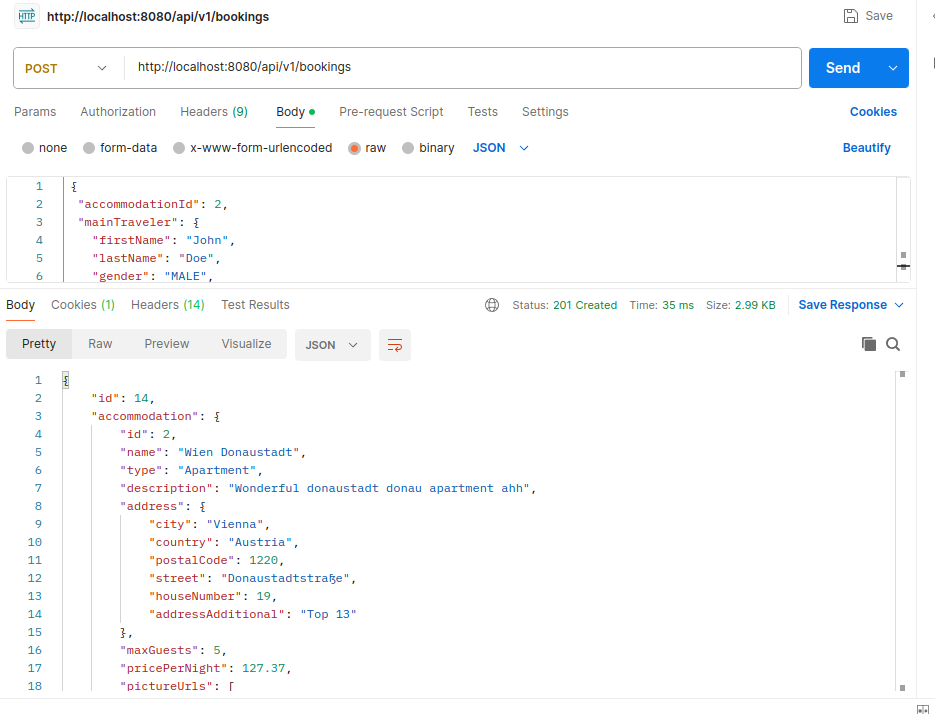
\includegraphics[width=1\textwidth]{images/impl-new-booking-post-req.png}
		\caption{Die Anfrage wurde erfolgreich abgeschickt und es wurde das gerade erstellte Objekt als JSON String zurückgegeben.}
        \label{req-bookings-post}
	\end{figure}
	
	Für das Testen der API-Schnittstellen wird Postman verwendet. Siehe \cite{website-postman}.
	
	Wie der Abbildung \ref{req-bookings-post} zu entnehmen ist, war die Anfrage erfolgreich. Wir haben den Status-Code 201 mit der Bedeutung \texttt{Created} zurückbekommen, das Objekt wurde also erfolgreich am Server erstellt und gespeichert.
	
	
	\subsubsection{Abrufen von Buchungen}
	
	Zum Abrufen von Buchungen wurden drei verschiedene Ansätze implementiert:
	\begin{enumerate}
		\item \textbf{getBookingById()}: Mit dieser Methode kann eine Buchung mit der exakten Buchungs-ID, welche in der Datenbank hinterlegt ist, abgerufen werden.
		\item \textbf{getAllBookings()}: Diese Methode ermöglicht das Abrufen aller gespeicherten Buchungseinträgen. Diese werden alle als JSON-String zurückgegeben.
		\item \textbf{getBookingsByAccommodation()}: Diese Methode wurde aufgrund des speziellen Use-Cases der Mitarbeiteransicht implementiert. Sie ermöglicht das Abrufen aller Buchungen, welche mit einer gewissen Unterkunft verknüpft sind. 
	\end{enumerate}
	
	Alle drei Ansätze haben etwas gemeinsam; sie lassen sich nicht einfach so im Internet aufrufen. Diese Methoden sind mittels Authentifizierung geschützt und es wird ein Mitarbeitertoken benötigt, um darauf zuzugreifen.
	
	\textbf{Abrufen einer Buchung mit der exakten Buchungs-ID}
	
	Der folgende Code-Ausschnitt repräsentiert die Logik hinter der Funktion, welche nur die Buchung mit der jeweiligen Buchungs-ID aufruft und zurückgibt:
	
	\begin{lstlisting}[caption={Aufrufen einer spezifischen Buchung mit der jeweiligen ID.}, label={code-bookings-get-booking}, language=Java]
		@PreAuthorize("isAuthenticated()")
		public ResponseEntity<Booking> getBookingById
		(@PathVariable("id") Long id) {
			Booking booking = bookingRepository.findById(id)
			.orElseThrow(() -> new ResourceNotFoundException());
			return ResponseEntity.ok(booking);
		}
	\end{lstlisting}
	
	In dem Code-Listing \ref{code-bookings-get-booking} wird als erstes sichergestellt, dass der Benutzer bzw. in diesem Fall der Mitarbeiter, der diese Buchung abrufen möchte, auch angemeldet ist. Wenn ein nicht angemeldeter Benutzer diese Schnittstelle aufruft, bekommt dieser einen \texttt{403-Fehler} (Forbidden). Die URL, um diese Methode aufzurufen, könnte lauten: \textit{https://example.com/api/v1/bookings/1}, wobei 1 für die ID des gewünschten Buchungs-Objektes steht. 
	
	\textbf{Abrufen aller Buchungen}
	
	Der folgende Codeblock \ref{code-bookings-get-all-bookings} zeigt die Funktionalität der Schnittstelle, alle gespeicherten Buchungen im JSON-Format auszugeben:
	
	\begin{lstlisting}[caption={Aufrufen aller in der Datenbank gespeicherten Buchungen.}, label={code-bookings-get-all-bookings}, language=Java]
		@PreAuthorize("isAuthenticated()")
		public ResponseEntity<List<Booking>> getAllBookings() {
			List<Booking> bookings = bookingRepository.findAll();
			return ResponseEntity.ok(bookings);
		\end{lstlisting}
		
		Dank dem \texttt{bookingRepository} ist das Laden aller Buchungen aus der Datenbank nur mit der \texttt{findAll()} Methode möglich. Dabei werden alle Buchungen in einer Liste vom Typ Booking gespeichert und dann zurückgegeben. Um diese Methode aufzurufen, genügt eine GET-Anfrage an die folgende URL: \newline
        \enquote{https://example.com/api/v1/bookings}.
		\newpage
		\textbf{Abrufen aller Buchungseinträge der jeweiligen Unterkunft}
		
		Nun gibt es auch noch die Möglichkeit, alle Buchungseinträge zu laden, welche an eine bestimmte Unterkunft geknüpft sind. 
		
		Dies wurde folgendermaßen implementiert:
		
		\begin{lstlisting}[caption={Aufrufen aller in der Datenbank gespeicherten Buchungen, welche mit der jeweiligen Unterkunft verknüpft sind.}, label={code-bookings-get-bookings-with-acc}, language=Java]
			Accommodation accommodation = accommodationRepository.findById(id)
			.orElseThrow(() -> new ResourceNotFoundException());
			List<Booking> bookings = bookingRepository
			.findByAccommodation(accommodation);
			return ResponseEntity.ok(bookings);
		\end{lstlisting}
		
		Der dargestellte Code im Listing \ref{code-bookings-get-bookings-with-acc} bekommt die ID der Unterkunft und durchsucht als Erstes die Datenbank danach, ob diese Unterkunft auch wirklich existiert. Falls nicht, wird ein \texttt{404-Error} geworfen.
		Als Nächstes werden dann alle Buchungs-Objekte aus der Datenbank gesucht, welche als Unterkunft (\texttt{Accommodation}) die übergebene und gefundene Unterkunft gesetzt haben.
		Das Abrufen dieser Methode lässt sich mit einer GET-Anfrage an die URL
		\enquote{https://example.com/api/v1/bookings/accommodation/1} bewerkstelligen, wobei 1 hierbei für die ID der Unterkunft stehen würde.
		
		\subsubsection{Beispiel-Anfrage: Abrufen aller Buchungen mit Unterkunft ID}
		
		Wir wollen uns nun alle Buchungen aus der Datenbank laden, welche im Zusammenhang mit der Unterkunft mit der ID = 2 stehen.
		
		Dafür muss folgendes vorhanden sein:
		
		\begin{enumerate}
			\item Der Benutzer muss angemeldet sein und einen gültigen Authentifizierungs-Token im Request Header übergeben.
			\item Die angegebene Unterkunft muss in der Datenbank existieren.
		\end{enumerate}
		
		\begin{figure}
			\centering
			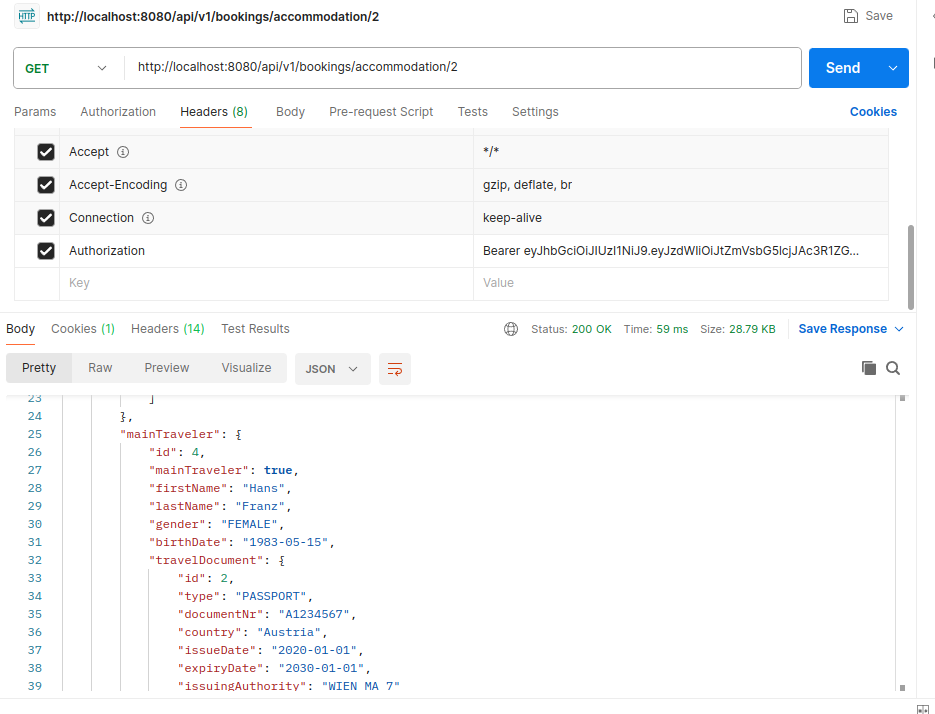
\includegraphics[width=1\textwidth]{images/impl-new-booking-get-acc-req.png}
			\caption{Die Anfrage wurde erfolgreich abgesendet und es wurden uns alle Buchungseinträge, welche mit der Unterkunft verknüpft sind, zurückgegeben.}
            \label{impl-new-booking-get-acc}
		\end{figure}
		
		Anhand der Abbildung \ref{impl-new-booking-get-acc} ist zu erkennen, dass die Anfrage erfolgreich war. Es wurden uns alle Buchungseinträge zurückgegeben, welche die Unterkunft mit der ID = 2 hinterlegt haben.
		
		\subsubsection{Aktualisieren und löschen von Buchungen}
		
		Die Operationen des Aktualisierens und Löschens der Buchungen basieren auf standardisierten Methoden, auf die nicht weiter eingegangen wird. Der vollständige Quellcode kann unter \cite{website-git-backend-repo} eingesehen werden.
		
		\subsection{API-Controller: Die Unterkunftsverwaltung}
		
		Neben der Buchungsverwaltung gibt es noch eine dedizierte Unterkunfts-Verwaltung, da diese einen essenziellen Teil im Workflow der Immobilienverwaltung von Equilibria darstellt. Dabei lassen sich neue Unterkünfte erstellen, abrufen, aktualisieren und löschen. Sicherheitstechnisch sind diese Schnittstellen weniger kritisch, da sie keine persönlichen oder sonstigen schützenswerten Daten beinhalten. Lediglich die Schreibvorgänge, also das Erstellen, Aktualisieren und das Löschen von Unterkünften, sind durch Authentifizierung geschützt. 
		
		\subsubsection{Erstellen einer Unterkunft}
		
		Um eine neue Unterkunft zu erstellen, werden die folgenden Daten benötigt:
		
		\begin{itemize}
			\item Name der Unterkunft
			\item Typ der Unterkunft (z.B. Haus, Wohnung, ...)
			\item Beschreibung
			\item Maximale Anzahl an gleichzeitigen Gästen
			\item Der Preis pro Nacht in €
			\item Die volle Adresse der Unterkunft
			\item (falls gewünscht) Eine Liste an Bild-URLS (kein direkter Image-Upload möglich)
		\end{itemize}
		
		Nun ist es möglich, als angemeldeter Mitarbeiter eine POST-Anfrage an die URL \break \enquote{https://example.com/api/v1/accommodations} mit den jeweiligen Daten zu machen. Für die vollständige Auflistung aller benötigten Daten siehe \cite{website-github-backend-example-accommodation-post}
		
		\begin{lstlisting}[caption={Überprüfung, ob die zu erstellende Unterkunft bereits in der Datebank existiert.}, label={code-acc-create-acc}, language=Java]
			@PostMapping
			@PreAuthorize("isAuthenticated()")
			public ResponseEntity<Accommodation> createAccommodation
			(@RequestBody AccommodationRequest accommodationRequest)  {
				if (accommodationRepository.findByName(accommodationRequest
				.getName()) != null) {
					throw new ConflictException();
				}
			\end{lstlisting}
			
			Als erstes wird hier in dem Listing \ref{code-acc-create-acc} überprüft, ob es bereits eine Unterkunft mit dem gleichen Namen in der Datenbank gibt. Falls dem so ist, wird eine sogenannte \texttt{ConflictException} (als ein Konflikt-Fehler) geworfen. Duplizierte Einträge können leicht vorkommen und Speicher und Performance negativ beeinflussen. Deshalb sind diese absolut zu vermeiden.
			
			\begin{lstlisting}[caption={Erstellung des Adress-Objektes für die Unterkunft}, label={code-acc-extract-info-out-of-body}, language=Java]
				Address address = new Address();
				address.setCity(accommodationRequest.getCity());
				[...]
				addressRepository.save(address);
			\end{lstlisting}
			
			Wie im Code-Listing \ref{code-acc-extract-info-out-of-body} zu sehen ist, werden im nächsten Schritt die Adressdaten aus dem Request Body extrahiert und in der Datenbank gespeichert.
			
			\begin{lstlisting}[caption={Erstellung eines neuen Accommodation-Objektes.}, label={code-acc-create-acc-objc}, language=Java]
			Accommodation accommodation = new Accommodation();
			accommodation.setAddress(address);
			accommodation.setName(accommodationRequest.getName());
			[...]
			accommodation.setPictureUrls(accommodationRequest.getPictureUrls());
			accommodationRepository.save(accommodation);
			return ResponseEntity.status(HttpStatus.CREATED).body(accommodation);
		\end{lstlisting}
		
		Dem Code-Listing \ref{code-acc-create-acc-objc} ist zu entnehmen, dass hier eine neue Instanz der Klasse Accommodation erstellt und initialisiert wird. Hier werden die zuvor erstellten und gespeicherten Adressdaten mit der Unterkunft assoziiert und sonstige Daten wie zum Beispiel die übergebenen Bild-Urls werden ebenso gesetzt.
		
		Schließlich wird die erstellte Unterkunft in der Datenbank gespeichert und es wird ein HTTP-Statuscode \texttt{200 - Created} inklusive dem gerade erstellten Objekt an den Client zurückgegeben.
		
		\subsubsection{Beispiel-Anfrage: Erstellung einer neuen Unterkunft}
		
		Wir möchten nun eine neue Unterkunft mit den folgenden Daten hinzufügen:
		
		\begin{itemize}
			\item Name: Villa Wien
			\item Type: Villa
			\item Beschreibung: Schöne Villa im 19. Wiener Gemeindebezirk
			\item Maximale Anzahl an gleichzeitigen Gästen: 20
			\item Preis pro Nacht: € 7849
			\item Adresse: Villastrasse 19, 1190 Wien, Österreich    
		\end{itemize}
		
		\begin{figure}
			\centering
			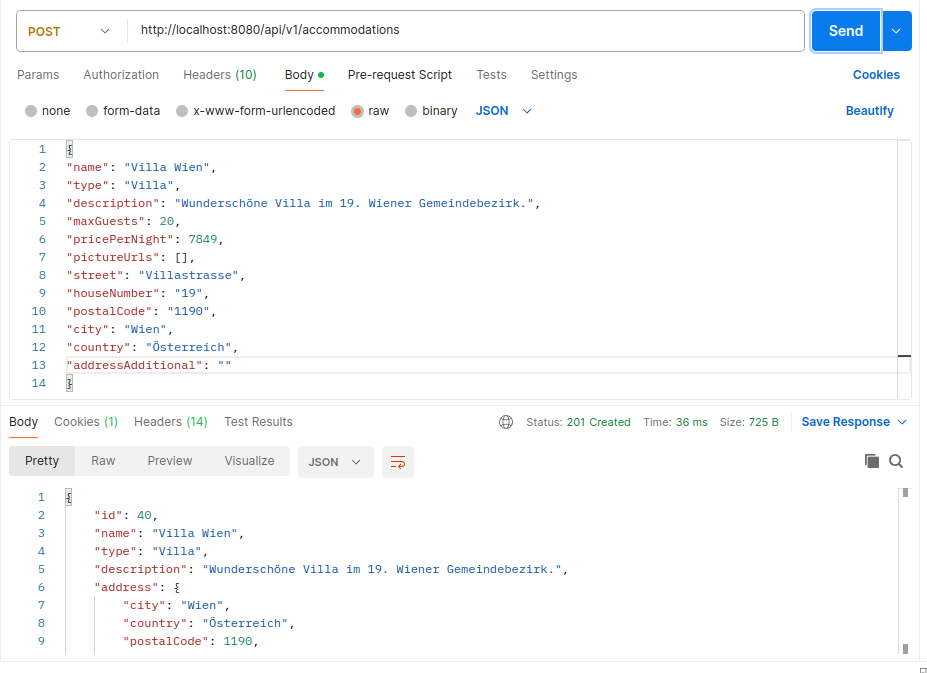
\includegraphics[width=1\textwidth]{images/impl-new-booking-post-acc-req.png}
			\caption{Die Anfrage wurde erfolgreich abgeschickt und es wurde uns der neu erstellte Accommodation-Eintrag zurückgegeben.}
            \label{impl-new-booking-post-acc-req}
		\end{figure}
		
		Wie in der Abbildung \ref{impl-new-booking-post-acc-req} zu sehen ist, war die Anfrage mit dem gesetzten Request Body erfolgreich. Das Accommodation-Objekt wurde erfolgreich erstellt und ist nun mit der ID = 40 in der Datenbank gespeichert. 
		
		\subsubsection{Abrufen, aktualisieren und löschen von Unterkünften}
		
		Die Operationen des Abrufens, Aktualisierens und Löschens der Unterkünfte basieren auf standardisierten Methoden, auf die nicht weiter eingegangen wird. Der vollständige Quellcode kann unter \cite{website-git-backend-repo} eingesehen werden.
		
		\subsection{Authentifizierung und Autorisierung}
		
		Die Implementierung der Authentifizierung und Autorisierung in dieser Anwendung basiert auf dem \gls{jwt} Standard. Dies ermöglicht eine sichere und effiziente Authentifizierung der Benutzer, insbesondere der Mitarbeiter des Auftraggebers, die Zugang zu geschützten Ressourcen benötigen. Anderenfalls wird dadurch unautorisierter Zugriff auf sensible Ressourcen vermieden.
		
		\subsubsection{JWT-Authentifizierung}
		
		Ein zentraler Bestandteil der Authentifizierung ist der \gls{jwt}, welcher nach erfolgreicher Anmeldung eines Benutzers generiert wird. Dieser Token wird für alle nachfolgenden Anfragen genutzt, um die Identität des Benutzers zu überprüfen. Die Logik für die Token-Verarbeitung ist in der Klasse \texttt{JwtService} implementiert. Siehe \cite{prompt-gpt-authentication-implementation}.
		
		\begin{lstlisting}[caption={Generierung eines JWT-Tokens für einen Benutzer.}, label={code-auth-create-jwt}, language=Java]
			public String generateToken(String username) {
				Map<String, Object> claims = new HashMap<>();
				return createToken(claims, username);
			}
		\end{lstlisting}
		
		
		Die Methode in \ref{code-auth-create-jwt} erzeugt ein JWT-Token mit dem übergebenen Benutzernamen und verwendet dabei eine Signatur, um die Integrität zu gewährleisten. 
		
		\begin{lstlisting}[caption={Validierung eines JWT-Tokens.}, label={code-auth-validate-jwt}, language=Java]
			public Boolean validateToken(String token, String username) {
				final String extractedUsername = extractUsername(token);
				return (extractedUsername.equals(username) && !isTokenExpired(token));
			}
		\end{lstlisting}
		
		Das Token wird bei jeder Anfrage an den Server überprüft, indem der Benutzername extrahiert und das Ablaufdatum validiert wird.
		
		\subsubsection{API-Controller: Registrierung}
		
		Die Registrierung eines neuen Mitarbeiters erfolgt über den Endpunkt \texttt{POST /api/v1/auth/register}. Dabei wird sichergestellt, dass nur autorisierte Personen neue Mitarbeiter registrieren können. Diese Funktionalität ist im \texttt{AuthController} vorhanden. Siehe \cite{prompt-gpt-authentication-implementation}.
		
		\begin{lstlisting}[caption={Validierung des Registrierungscodes bei der Anmeldung eines neuen Mitarbeiters.}, label={code-auth-employee-reg}, language=Java]
			if (!isValidUniqueCode(registerRequest.getUniqueCode())) {
				throw new BadRequestException("Invalid registration code provided");
			}
		\end{lstlisting}
		
		Dem Code-Listing \ref{code-auth-employee-reg} zu entnehmen ist der Anfang des Registrierungs-Prozesses. Als Erstes wird überprüft, ob der sogenannte \texttt{Unique Registration Code} korrekt ist. Dies ist ein Passwort, welches von der Firma lokal auf dem Server gesetzt wird. Nur mit diesem Passwort ist ein Registrierungsvorgang möglich.
		
		\begin{lstlisting}[caption={Erstellung eines neuen Mitarbeiter-Accounts.}, label={code-aut-employee-reg-2}, language=Java]
			Employee newEmployee = new Employee();
			newEmployee.setUsername(registerRequest.getUsername());
			newEmployee.setPassword(passwordEncoder.encode(registerRequest.getPassword()));
			newEmployee.addRole(Roles.EMPLOYEE);
			employeeRepository.save(newEmployee);
		\end{lstlisting}
		
		In dem Codeblock \ref{code-aut-employee-reg-2} wird ein neues Employee-Objekt mit dem gegebenen Benutzernamen und Passwort erstellt. Hierbei wird das Passwort mit der von Spring Boot Security bereitgestellten \texttt{PasswordEncoder.encode()} Methode gehasht und erst dann in die Datenbank gespeichert. Diese Speicherung stellt sicher, dass die Daten der Mitarbeiter nicht im Klartext in der Datenbank vorhanden sind – was ein enormes Sicherheitsrisiko wäre.
		
		Danach wird dem Mitarbeiter noch die \texttt{EMPLOYEE}-Rolle zugeteilt. Dies ist die Default-Rolle, welche alle Mitarbeiter des Auftraggebers bekommen. Ebenso wird im Code noch der zur Registrierung verwendete Unique Registration Code gespeichert, um mögliche Missbräuche des Codes sofort aufdecken zu können.
		
		\subsubsection{API-Controller: Login}
		
		Die Anmeldung erfolgt über den Endpunkt \texttt{POST /api/v1/auth/login}. Diese Funktionalität ist im \texttt{AuthController} vorhanden. Bei der Anmeldung muss ein valider Benutzername und ein valides Passwort eines existierenden Mitarbeiters angegeben werden. Siehe \cite{prompt-gpt-authentication-implementation}.
		
		\begin{lstlisting}[caption={Validierung der Benutzereingaben beim Login.}, label={code-auth-login-req}, language=Java]
			@PostMapping("/login")
			public ResponseEntity<?> login(@RequestBody LoginRequest loginRequest,
			HttpServletRequest request) {
				if (loginRequest.getUsername() == null || 
				loginRequest.getPassword() == null) {
					throw new BadRequestException();
				}
			\end{lstlisting}
			
			Hier, im Listing Nr. \ref{code-auth-login-req}, wird überprüft, ob die benötigten Daten angegeben wurden.
			Sofern ein Benutzername und Passwort angegeben wurden, wird der Mitarbeiter in der Datenbank gesucht und das Passwort überprüft.
			
			In dem folgenden Codeblock wird der Mitarbeiter aus der Datenbank geladen und es werden die Passwörter überprüft. Hierfür wird ebenso die von Spring Boot Security bereitgestellte \texttt{PasswortEncoder.matches()} Methode verwendet. Diese Methode ist kryptografisch sicher, da sie das gegebene Passwort hasht und diesen Hash dann mit dem gespeicherten Passwort-Hash in der Datenbank vergleicht. Somit kann im Programm das Passwort während des Vergleichs nicht extrahiert werden.
			
			\begin{lstlisting}[caption={Passwortprüfung und Token-Generierung bei erfolgreichem Login.}, label={code-auth-process-login-req}, language=Java]
				Employee employee = employeeRepository
				.findByUsername(loginRequest.getUsername());
				if (employee != null && passwordEncoder
				.matches(loginRequest.getPassword(), employee.getPassword())) {
					return ResponseEntity.ok().body(jwtService
					.generateToken(employee.getUsername()));
				}
				throw new BadRequestException("Invalid credentials were provided");
			\end{lstlisting}
			
			Falls das Passwort korrekt ist, wird eine HTTP-Request mit dem Status \texttt{200 - OK} mit dem JWT im Request Body zurückgegeben. Mit diesem Token kann der Mitarbeiter die geschützten Daten aus dem Backend abfragen. Dieser Prozess läuft automatisch im Frontend ab.
			
			\subsubsection{JWT-Filterung und Sicherheitsmechanismen}
			
			Um sicherzustellen, dass jede Anfrage authentifiziert ist, wird ein JWT-Filter genutzt, der die Tokens aus den Anfragen extrahiert und validiert. Siehe \cite{prompt-gpt-authentication-implementation}.
			
			\begin{lstlisting}[caption={Extrahierung des JWT-Tokens aus dem Authorization-Header.}, label={code-auth-jwt-service-extract-token}, language=Java]
				final String authHeader = request.getHeader("Authorization");
				if (authHeader == null || !authHeader.startsWith("Bearer ")) {
					filterChain.doFilter(request, response);
					return;
				}
			\end{lstlisting}
			
			
			Im Code-Listing Nr. \ref{code-auth-jwt-service-extract-token} wird der Code-Ausschnitt dargestellt, welcher überprüft, ob der Autorisationstoken im Request-Header enthalten ist. Dieser muss in der Form \texttt{Authorization: Bearer <token>} vorhanden sein, ansonsten wird die Anfrage sofort abgebrochen und es wird ein \texttt{403 - Forbidden} Status zurückgegeben.
			
			\begin{lstlisting}[caption={Validierung des JWT-Tokens und Setzen der Authentifizierung im Spring-Kontext.}, label={code-auth-jwtservice-validate-token}, language=Java]
				if (jwtService.validateToken(jwtToken, userDetails.getUsername())) {
					UsernamePasswordAuthenticationToken authToken =
					new UsernamePasswordAuthenticationToken(userDetails, null
					, userDetails.getAuthorities());
					SecurityContextHolder.getContext()
					.setAuthentication(authToken);
				}
			\end{lstlisting}
			
			Falls der Token, welcher übergeben wurde, gültig ist, wird die Benutzeridentität im Spring-Kontext gesetzt. Das heißt, dass die ganze Applikation nun weiß, wer dieser Benutzer ist. Es kann hiermit auch im gesamten Programm mit dieser Identität gearbeitet werden.

            \newpage
			
			\subsubsection{Spring-Security Konfigurationen}
			
			Zusätzlich zu den bis jetzt genannten Sicherheitsmaßnahmen werden ebenso Spring-Interne Sicherheitskonfigurationen gesetzt. Diese sind in der \texttt{SecurityConfig} enthalten.
			
			\begin{lstlisting}[caption={Initialisierung von allgemeinen Security-Konfigurationen wie dem Passwort-Encoder.}, label={code-spring-sec-conf-1}, language=Java]
				@Configuration
				@EnableWebSecurity
				public class SecurityConfig {
					@Autowired
					private JwtAuthenticationFilter jwtAuthenticationFilter;
					@Autowired
					private CustomUserDetailsService customUserDetailsService;
					@Bean
					public PasswordEncoder passwordEncoder() {
						return new BCryptPasswordEncoder();
					}
				\end{lstlisting}
				
				Das Code-Listing \ref{code-spring-sec-conf-1} stellt den Anfang der Security-Konfiguration von Spring Boot Security dar. Mittels \texttt{@Configuration} und \texttt{@EnableWebSecurity} deklarieren wir alles in dem File als Spring Konfiguration und aktivieren das Web-Security-Plugin.
				
				\begin{lstlisting}[caption={Erstellung der SecurityFilterChain in Spring Boot.}, label={code-spring-sec-conf-2}, language=Java]
					@Bean
					public SecurityFilterChain securityFilterChain(HttpSecurity http) {
						http.csrf(AbstractHttpConfigurer::disable)
						.cors(cors -> cors.configurationSource(corsConfigurationSource()))
						.authorizeHttpRequests(auth -> auth
						.requestMatchers("/api/v1/auth/login").permitAll()
						.requestMatchers("/api/v1/auth/register").permitAll()
					\end{lstlisting}
					
					In diesem Code-Listing Nr. \ref{code-spring-sec-conf-2} wird die sogenannte \texttt{SecurityFilterChain} in Spring Boot erstellt und zum Teil eingerichtet. Diese \enquote{Kette} ist für die Abarbeitung von Anfragen zuständig. Jede Anfrage, welche in den Server eingeht, muss als Erstes durch diese Filter-Chain gehen. 
					
					Wichtige Kriterien bei dieser Filter-Kette sind, dass:
					
					\begin{itemize}
						\item \gls{cors} ist aufgrund von Entwicklungsgründen noch aktiviert.
						\item \gls{csrf} ist aufgrund der hohen Sicherheitsrisiken deaktiviert. Siehe \cite{website-csrf-explanation}.
						\item Ebenso wurden explizit die zwei API-Pfade \texttt{/api/v1/auth/login} sowie \texttt{/api/v1/auth/register} freigegeben. Das bedeutet, dass jeder diese Endpunkte erreichen kann.
					\end{itemize}
					
					Da dies nur ein Teil der Konfiguration war, kommen wir nun zum restlichen Teil der Sicherheitskonfiguration:

                    \newpage
                    
					\begin{lstlisting}[caption={Fertigstellung der Definition der SecurityFilterChain in Spring Boot.}, label={code-spring-sec-conf-3},language=Java]
						.requestMatchers(HttpMethod.POST, "/api/v1/bookings")
						.permitAll()
						.requestMatchers(HttpMethod.GET, "/api/v1/accommodations")
						.permitAll()
						.requestMatchers(HttpMethod.GET, "/api/v1/accommodations/{id}")
						.permitAll()
						.anyRequest().authenticated()
						)
						http.addFilterBefore(jwtAuthenticationFilter, 
						UsernamePasswordAuthenticationFilter.class);
					}
				\end{lstlisting}
				
				In diesem Teil der Filter-Chain legen wir ebenso wichtige Konfigurationen fest:
				
				\begin{itemize}
					\item Die URL \texttt{/api/v1/bookings} darf nur als POST-Request unautorisiert erreicht werden. Dies dient dazu, damit sich der Mieter für das Ausfüllen des Formulars keinen extra Account oder Ähnliches erstellen muss.
					\item Ebenso dürfen die URLs \texttt{/api/v1/accommodations} sowie \texttt{/api/v1/accommodations/{id}} unautorisiert verwendet werden. Da diese Endpunkte keine Auskunft über sensible Informationen geben, ist dies sicherheitstechnisch auch unbedenklich.
					\item Danach wird durch \texttt{anyREquest().authenticated()} noch die Richtlinie gesetzt, dass jede Anfrage, welche nicht in das gerade genannte Muster passt, authentifiziert sein muss. 
					\item Schließlich wird durch \texttt{http.addFilterBefore()} noch unser vorher definierte JWT Authentication Filter hinzugefügt.
				\end{itemize}
				
				Diese Sicherheitsmaßnahmen sorgen für eine zuverlässige Authentifizierung und Autorisierung, indem sie sicherstellen, dass nur registrierte und berechtigte Benutzer auf geschützte Ressourcen zugreifen können.
				\subsection{Datenschutz und Sicherheit}
				
				\subsubsection{Speicherung und Schutz sensibler Daten}
				
				Zur Sicherheit und Nachverfolgbarkeit von Anmelde- und Zugriffsvorgängen werden die Klassen \texttt{AccessLogService} und \texttt{LoginLogService} genutzt. Diese speichern zum einen Anmeldungen aller Mitarbeiter inklusive UserAgent und IP-Adresse sowie relevante Zugriffe auf die API-Schnittstellen. Diese Einträge werden dann in der Datenbank archiviert.
				
				\subsubsection{Schutz personenbezogener Daten}
				
				Die Anwendung hält sich an die Datenschutz-Grundverordnung (DSGVO), indem personenbezogene Daten nur verschlüsselt gespeichert und verarbeitet werden. Sensible Informationen wie Passwörter werden mit einem sicheren Hashing-Algorithmus (BCrypt) gehasht, um unautorisierten Zugriff zu verhindern.
				
				\subsubsection{Zugriffskontrollen}
				
				Die Anwendung nutzt ein rollenbasiertes Zugriffskontrollsystem (RBAC), um sicherzustellen, dass nur autorisierte Benutzer bestimmte Aktionen durchführen können. Rollen wie \texttt{EMPLOYEE} und \texttt{ADMIN} definieren unterschiedliche Berechtigungen für die Nutzung der API-Endpunkte. Siehe \cite{prompt-gpt-datenschutz-implementation}.
				
				\subsection{Fehlerbehandlung}
				
				Es wurde eine eigene Exception-Handling-Struktur implementiert, um zu verhindern, dass dem Benutzer eventuell echte und ausschlaggebende Fehlermeldungen mit eventuellen Stacktraces angezeigt werden. Dies stellt ein großes Sicherheitsrisiko dar, da dem Benutzer in so einem Moment Einblick in das Innere der Applikation gewährt wird. Dadurch können eventuell sensible Daten ausgegeben werden. Diese Exception-Handling Struktur ist im \texttt{GlobalExceptionHandler} zu finden.
				
				\subsubsection{Globale Fehler}
				
				Globale Fehler in der Applikation, also Fehler, welche entweder nicht identifiziert werden konnten oder von externen Anbietern geworfen werden, werden als \enquote{generelle Exceptions} bezeichnet. Diese werden immer mit dem Status-Code \texttt{500 - Internal Server error} und der Fehlernachricht \enquote{An unexpected error occurred} ausgegeben. 
				
				Implementiert wird dieser Handler im Code folgendermaßen:
				
				\begin{lstlisting}[caption={Der Globale Fehler-Handler.}, label={code-global-exc-handler}, language=Java]
					@ExceptionHandler(Exception.class)
					public ResponseEntity<ErrorResponse> handleGeneralException(Exception ex) {
						ErrorResponse errorResponse = new ErrorResponse(
						LocalDateTime.now(), HttpStatus.INTERNAL_SERVER_ERROR.value(),
						"An unexpected error occurred."
						);
						return new ResponseEntity<>(errorResponse,
						HttpStatus.INTERNAL_SERVER_ERROR);
					}
				\end{lstlisting}
				
				Wie in dem Code-Listing Nr. \ref{code-global-exc-handler} zu sehen ist, werden hier alle globalen Fehler, welche nicht identifiziert oder sonst zugeordnet werden konnten, überarbeitet und ausgegeben. 
				
				\subsubsection{Applikationsspezifische Fehler}
				
				Neben den globalen Fehlern gibt es auch applikationsspezifische Fehler, welche die Usability verbessern sollen. 
				Darunter fallen die folgenden Exception-Klassen:
				
				\begin{itemize}
					\item \textbf{BadRequestException}: Wird geworfen, wenn der Server eine Anfrage bekommt, welche nicht alle für die weitere Verarbeitung notwendigen Parameter besitzt.
					\item \textbf{ConflictException}: Wird bei Datenbank-Duplikaten geworfen, da hier ein Konflikt entsteht.
					\item \textbf{ProtocolGenerationException}: Wird geworfen, wenn während der Generierung der Buchungsprotokolle fehler auftreten.
					\item \textbf{ResourceNotFoundException}: Wird geworfen, wenn eine angefragte Ressource auf dem Server nicht existiert.
					\item \textbf{UnauthorizedException}: Wird geworfen, wenn eine Ressource ohne die notwendige Authentifizierung aufgerufen wird.
				\end{itemize}
				
				\subsection{Zusammenfassung der Implementierung}
				
				\subsubsection{Reflexion der Herausforderungen}
				
				Während der Implementierung traten verschiedene Herausforderungen auf, insbesondere in den Bereichen Authentifizierung, Zugriffskontrolle und Fehlerbehandlung. Die korrekte Integration von Spring Security mit JWT stellte sich als komplizierter heraus, als ursprünglich gedacht, da unterschiedliche API-Endpunkte verschiedene Sicherheitsstufen benötigten.
				
				Ein weiteres Problem war das Exception Handling. Um sicherzustellen, dass Fehler nicht zu sensiblen Datenlecks führen, wurde ein \texttt{GlobalExceptionHandler} entwickelt, der kontrollierte Fehlermeldungen ausgibt und sicherheitskritische Details verbirgt.
				
				Schließlich war die größte Herausforderung das Paket-Management. Denn besonders hier ist es aufgrund von veralteten Versionen, verschobenen Paketen, uvm. oft zu Konflikten gekommen. Die Fehlernachrichten dieser Art von Fehlern waren sehr schwer zu interpretieren. Schließlich wurde eine einheitliche Struktur geschaffen, welche sich auch auf allen Betriebssystemen ausführen lässt. Siehe \cite{prompt-gpt-reflexion-implementation}.
				
				\subsubsection{Ausblick für mögliche Erweiterungen}
				
				Für zukünftige Versionen sind folgende Erweiterungen denkbar:
				
				\begin{itemize}
					\item \textbf{Feingranulare Zugriffskontrolle}: Detailliertere Implementierung des Role-Based Access Systems, um differenziertere Berechtigungsstrukturen zwischen den jeweiligen Rollen einführen zu können.
					\item \textbf{Erweiterte Protokollierung}: Ausbau der AccessLog- und LoginLog-Datenbank zur detaillierteren Analyse von Zugriffsmustern und Sicherheitsereignissen. Eventuell wäre hier eine automatische Auswertung der Zugriffe möglich, was den Sicherheitsfaktor noch einmal erhöht.
					\item \textbf{Caching-Struktur}: Die Implementierung einer Caching-Struktur würde die Performance der API besonders bei enorm großen Datenmengen um einiges erhöhen. 
					\item \textbf{Automatisierte Tests}: Ausbau von Unit- und Integrationstests zur Erhöhung der Stabilität und Reduzierung von Fehlerquellen in zukünftigen Versionen.
				\end{itemize} Siehe \cite{prompt-gpt-reflexion-implementation}.